\documentclass[11pt, oneside]{article} 
\usepackage{geometry}
\geometry{letterpaper} 
\usepackage{graphicx}
	
\usepackage{amssymb}
\usepackage{amsmath}
\usepackage{parskip}
\usepackage{color}
\usepackage{hyperref}

\graphicspath{{/Users/telliott/Github/calculus_book/png/}}
% \begin{center} \includegraphics [scale=0.4] {gauss3.png} \end{center}

\title{Primes}
\date{}

\begin{document}
\maketitle
\Large

\subsection*{prime numbers}
As you know, the positive integers larger than $1$ are of two types:

$\bullet$ \ a prime number $p$ has only two factors, $p$ itself and $1$

$\bullet$ \ a composite number has at least one additional factor.  Either the number is a perfect square of a prime, or it has an even number of additional factors: $a_1 \dots a_k$.

The first ten primes are:
\begin{verbatim}
2 3 5 7 11 13 17 19 23 29 ...
\end{verbatim}

\subsection*{The sieve of Eratosthenes}

Eratosthenes is famous in mathematics for his "sieve" which allows one to determine which numbers are prime in an economical fashion.  

We will take note of him again in talking about the circumference of the earth.  He was a contemporary of Archimedes and became the chief librarian at the Library of Alexandria when he was only about 35 years old.

The sieve operates by first writing down all the integers to some upper limit (here $120$).  To carry out the process manually it is convenient to use rows with $10$ values, so there are $12$ rows in all here.  Most of the boxes have not yet been numbered (below, left).

Starting with the first prime number, $2$, eliminate all the numbers divisible by $2$ (all the red numbers, or even numbers).  Here this has been done by coloring red all squares with numbers ending in $2,4,6,8,0$.

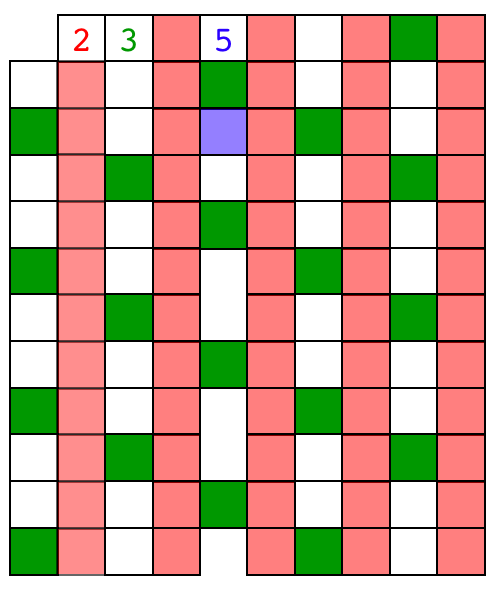
\includegraphics [scale=0.3] {sieve6.png}
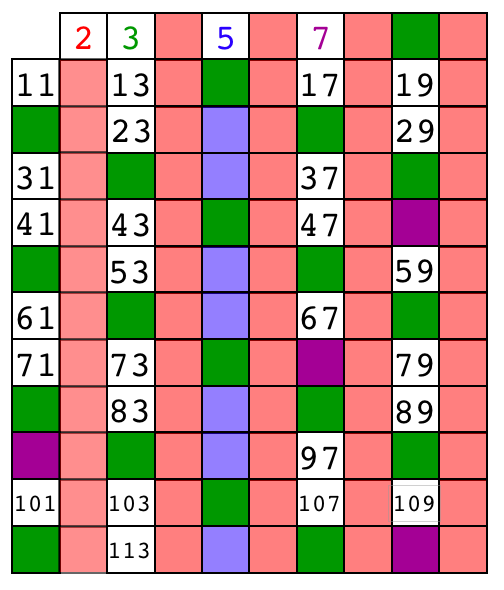
\includegraphics [scale=0.3] {sieve7.png}

Next, do the same thing with $3$ (green).  $6$ was already eliminated previously, but odd multiples of $3$ like $9$, $15$ and $21$ go away at this step.

The next larger number that still has a white square is $5$.  All the squares eliminated at this step are white ones in the fifth row, starting with $25$.  Continue with $7$, eliminating $49, 77, 91$ and $119$.

The sieve now ends (for this upper bound of $120$).  

The rule is that if the number for the next round, the smallest number not yet eliminated, is larger than the square root of the upper limit ($\sqrt{120}$), we terminate.  

So $7$ is the last value used, because after that round the smallest remaining integer is $11$, but we terminate since $11^2 = 121 > 120$.

The graphic shows all the numbers which have yet to be eliminated after the round of $7$.   All of these numbers, $11$, $13$, $17$, and so on, as well as those used as divisors for each round of the sieve ($2, 3, 5, 7$), are prime numbers.

By testing for division by $2, 3, 5$ and $7$, we have found the first $30$ prime numbers.

\begin{verbatim}
 2   3   5   7  11  13  17  19  23  29
31  37  41  43  47  53  59  61  67  71 
73  79  83  89  97 101 103 107 109 113
\end{verbatim}

From a performance standpoint, it is important that we do not need to carry out division.  All that is really needed is repeated addition.  Coding this algorithm in, say, Python is a good challenge.  

A bigger challenge is to come up with a method to \emph{grow} the list of primes on demand.  This can be done by keeping track of the first value to be tested above the limit, for each prime in the current list.

\subsection*{recognizing primes quickly}

There are school problems that require you to factor numbers at least up to $100$, maybe more, quickly.  It can be helpful to learn to recognize the primes in this range.

$\circ$ \ First, primes end in one of the digits: $1,3,7,9$.

$\circ$ \ Test quickly for $3$ as a factor by the digit sum trick.

$\circ$ \ Test $7$ as a factor by trial multiplication.

Let's do the first row, for an example:
\begin{verbatim}
11 21 31 41 51 61 71 81 91 101 111
\end{verbatim}

You should recognize $11$ as prime, immediately.  Then remove the numbers whose digits add up to $3$ or a multiple, leaving

\begin{verbatim}
31 41 61 71 91 101
\end{verbatim}

Then, trial multiplication by $7$ to get a number ending in $1$.  

The $1$ reminds me of $21$, so I guess:  $7 \cdot (10 + 3) = 70 + 21 = 91$.  Gone.

$\circ$ \ $91 - 71 = 20$

$\circ$ \ $91 - 61 = 30$

$\circ$ \ $101 - 91 = 30$

$\circ$ \ $91 - 41 = 50$

None of these differences is divisible by $7$, so the numbers are not, either.

I trust you recognize that $31$ is $3$ more than $7 \cdot 4$.

We do not need to test any primes larger than $11$.  All multiples of $11$ are double digits, until $110$.  

That leaves:

\begin{verbatim}
31 41 61 71 101
\end{verbatim}

\begin{center}
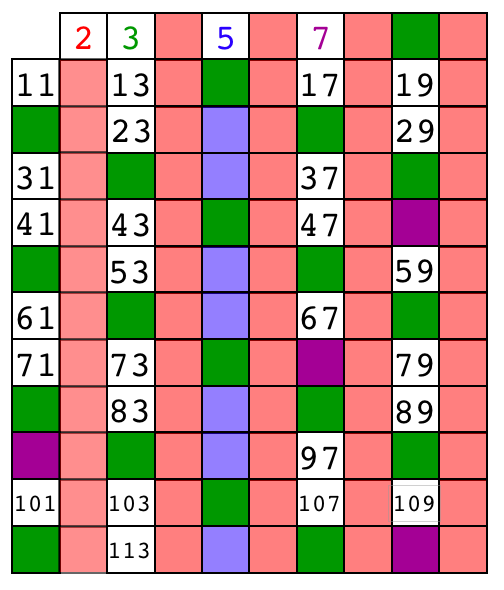
\includegraphics [scale=0.3] {sieve7.png}
\end{center}



\subsection*{infinite primes}

Euclid has a theorem and a proof that the number of primes is infinite.

Proof:

By contradiction.

Suppose the set of primes is finite, and that $p_1$, $p_2 \dots p_k$ are all of the primes.  Construct the following numbers:
\[ P = (p_1 \cdot p_2 \cdot \dots p_k)  \]
\[ Q = P + 1 \]
For a prime number $p$ to evenly divide $Q$, it must divide the difference between $Q$ and $P$.  But that difference is $1$ and so can't be divided evenly by any prime.

Therefore, none of the known primes divides $Q$ and at least one of these is true:

$\bullet$ \  $Q$ is a prime not in the set of known primes

$\bullet$ \ the set was originally incomplete

The assumption that the set of primes is finite leads to a contradiction.

$\square$

Even for a relatively small number of primes, we may encounter the second situation.  Start with the first prime:  $2$:
\[ 2 + 1 = 3 \ \text{(prime)} \]
\[ 2 \cdot 3 + 1 = 7 \ \text{(prime)}  \]
\[ 2 \cdot 3 \cdot 7 +1 = 43 \ \text{(prime)}  \]
\[ 2 \cdot 3 \cdot 7 \cdot 43 + 1 =  1807 \]
$1807$ is \emph{not} prime.  ($1807 = 13 \cdot 139$).

\subsection*{testing primality}
This is a pretty deep subject.  However, a simple filter to apply first is to ask:  is the last digit one of $\{ 0,2,4,6,8 \}$, i.e. is the number even?  Does the number end in $5$?  Or is the sum of the digits divisible by $3$ or $9$?

There is a trick for the last test.  If a number is divisible by $3$ its digits add to a multiple of three.  Suppose the number is:
\[ abcd = a \cdot 10^3 + b \cdot 10^2 + c \cdot 10^1 + d \]
\[ = a (9 \cdot 10^2 + 1) + b (9 \cdot 10^1 + 1) + c (9 \cdot 10 + 1) + d \]
If $x|(y+z)$ and $x|y$ then it must be that $x|z$.  Since $9$ times anything is divisible by $3$, it follows that $3$ must divide $a + b + c + d$ for $abcd$ to be divisible by $3$.

A similar thing is true of $9$ except that the digits must add only to $9$.

A more general observation is that all primes greater than $3$ are of the form $4k + 1$ or $4k + 3$, for integer $k$.  That's because $4k$ and $4k + 2$ are even, and $4k + 4 = 4(k + 1)$.

Any composite number $n$ has a unique prime factorization.  Its smallest prime factor $p$ has the property (easily proved):
\[ p^2 \le n \]

Therefore, it suffices to check whether the prime numbers less than or equal to the square root of $n$ divide $n$.  If the square root is not an integer, we need check only the next smallest integer, what is called the \emph{floor} of the value.  If no prime less than that divides $n$, then $n$ is a prime.

This can be improved still more.

\url{https://en.wikipedia.org/wiki/Primality_test}


\end{document}